\section{System Context}\label{sec:1}

\subsection{Business Context}\label{sec:1.1}

VinaBeef Livestock Joint Stock Company operates large-scale beef cattle
farms in Dak Lak, Gia Lai and Dong Nai, with a standing herd of
approximately 25,000 cattle across 120 barns. Every animal wears a
unique RFID ear tag that serves as its permanent identifier for its
whole life on the farm.

Each barn has RFID gate readers at its entrances and exits. When cattle
pass through a gate, for example leaving for grazing or returning to the
barn, the reader records the animal' s identity and the
timestamp as a movement transaction, without manual work.

\subsection{Problem Statement}\label{sec:1.2}

\begin{itemize}
\item
  Manual head counts at this herd size are slow and error-prone, which delays the detection of missing or stray cattle.
\item
  Vaccination, treatment and movement records kept in separate places prevent a complete history for each animal.
\item
  Manual reporting to the National Animal Disease Control System delays disease surveillance; the assignment requires this exchange to use an API.
\item
  Management needs consolidated monitoring across the three farms, with data
  freshness and provisional/offline states visible.
\end{itemize}

These problems are derived from the assignment description, which does
not document VinaBeef's current manual process in detail.

\subsection{Objectives}\label{sec:1.3}

{\small
\begin{longtable}[]{|>{\raggedright\arraybackslash}p{\dimexpr 0.0753\linewidth-2\tabcolsep\relax}|>{\raggedright\arraybackslash}p{\dimexpr 0.4299\linewidth-2\tabcolsep\relax}|>{\raggedright\arraybackslash}p{\dimexpr 0.4649\linewidth-2\tabcolsep\relax}|}
\hline
\textbf{ID} & \textbf{Objective} & \textbf{Measure} \\ \hline
\endhead
\textbf{O1} & Automate movement recording at barn gates & 100\% of gate
passages recorded without manual input \\ \hline
\textbf{O2} & Detect abnormal situations quickly & Missing/unexpected
animals alerted within the configured window \\ \hline
\textbf{O3} & Keep a complete lifetime profile per animal & Vaccination,
health, treatment and movement history in one place \\ \hline
\textbf{O4} & Support regulatory health surveillance & Required data
sent to the National system through its API \\ \hline
\textbf{O5} & Ensure security and accountability & Role-based access;
every change audited \\ \hline
\end{longtable}
}

\subsection{Scope}\label{sec:1.4}

\textbf{In scope:} cattle and RFID tag management; barn, gate and reader
management; automated in/out movement recording and counting;
abnormality detection and alerting; vaccination, health and movement
history; reporting and auditing; system administration.

\textbf{Out of scope (this phase):} feed and nutrition management; sales
and slaughter traceability. The system manages only live-animal
identification, movement and health data within the farms.

\subsection{Assumptions and Constraints}\label{sec:1.5}

\begin{itemize}
\item
  Every animal is tagged with a unique, readable RFID ear tag before
  entering the system.
\item
  Farms are in rural areas; internet connectivity to the central site
  can be slow or interrupted.
\item
  Each gate has reader hardware able to determine passing direction (for
  example, two antennas or a reader pair).
\item
  The National Animal Disease Control System exposes an API for
  submitting outbreak and health surveillance data.
\item
  Peak load: about 200 cattle pass the gates of one farm within 30
  minutes during herd release or return.
\end{itemize}

\subsection{Stakeholders and Actors}\label{sec:1.6}

{\small
\begin{longtable}[]{|>{\raggedright\arraybackslash}p{\dimexpr 0.2794\linewidth-2\tabcolsep\relax}|>{\raggedright\arraybackslash}p{\dimexpr 0.1719\linewidth-2\tabcolsep\relax}|>{\raggedright\arraybackslash}p{\dimexpr 0.5187\linewidth-2\tabcolsep\relax}|}
\hline
\textbf{Actor} & \textbf{Type} & \textbf{Main goals} \\ \hline
\endhead
\textbf{Barn Supervisor} & Primary & Monitor head count, respond to
alerts, record health events in their barns \\ \hline
\textbf{Farm Manager} & Primary & Oversee all barns of a farm, manage
transfers, review reports \\ \hline
\textbf{System Administrator} & Primary & Manage users, roles, devices
and configuration \\ \hline
\textbf{Executive Management} & Primary & Monitor dashboards and
company-wide reports \\ \hline
\textbf{RFID Gate Reader} & System actor & Send tag read events
automatically \\ \hline
\textbf{National Animal Disease Control System} & External system &
Receive outbreak and health surveillance data \\ \hline
\end{longtable}
}

\begin{figure}[htbp]\centering
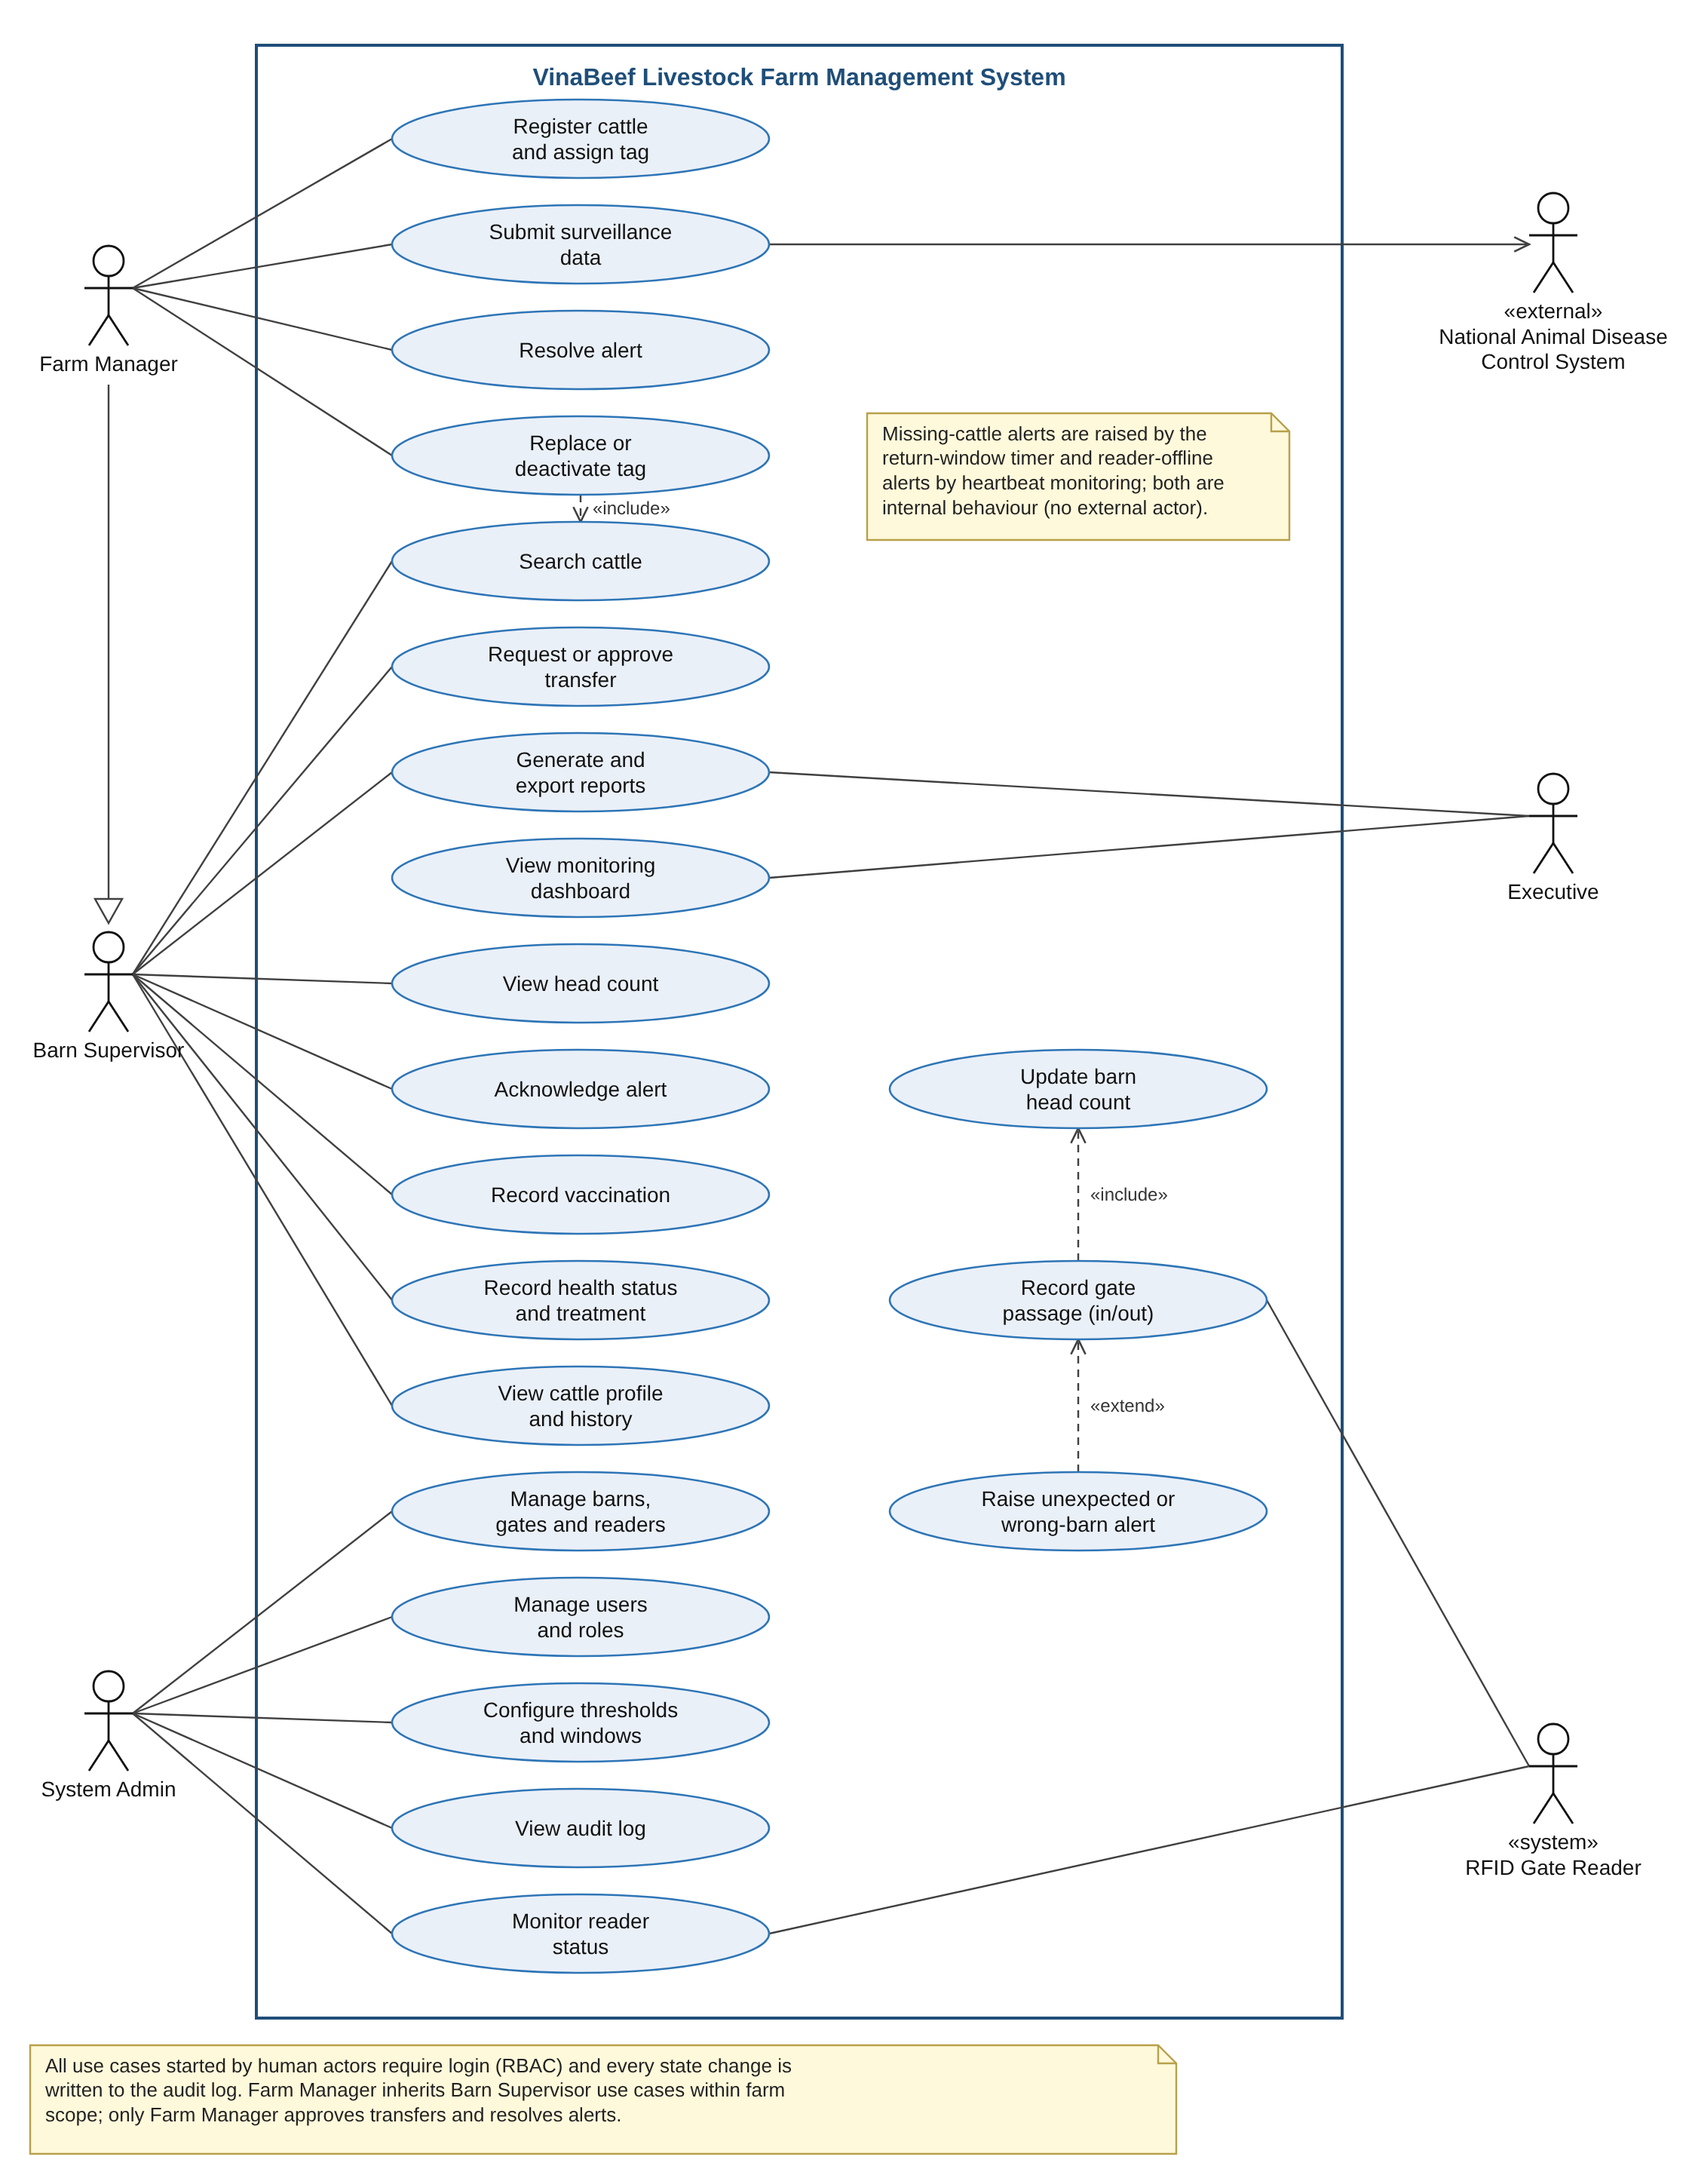
\includegraphics[width=\linewidth,height=0.8\textheight,keepaspectratio]{graphics/vinabeef/fig01-use-case-diagram.png}
\caption{Use case diagram}\label{fig:1}\end{figure}
